\documentclass[]{article}
\usepackage[table, dvipsnames]{xcolor}% http://ctan.org/pkg/xcolor
\usepackage{fullpage} % Package to use full page
\usepackage{parskip} % Package to tweak paragraph skipping
\usepackage{tikz} % Package for drawing
\usepackage{amsmath}
\usepackage{hyperref}




\title{Introduction to Adafruit and the LCD Display  --  Hello, World!}
\author{Dr. Matthew Riehl}


\begin{document}

\newcommand{\tc}{\textcolor}

\maketitle
%{today}

\section{Introduction}

For the next several weeks, we will be building circuits to investigate the properties of resistors, capacitors,  and other electronic components.  In order to do this, we  first build a simple device that will be used to help us gather our data in later labs.

\emph{Note that this is NOT a programming class (no previous programming experience is needed); the code is provided and can be used without editing (although you are encouraged to play with the code to extend the functionality of the device\dots). Neither is this a circuits class; we will not be exploring the details of how the Arduino and other components work.  Of course, we hope that this taste of programming and bread-boarding inspire you to take additional courses in computer science or electronics\dots}

This week, we will set up the Adafruit Metro Express to send a  message to the LCD display.  You will wire the LCD to the Metro Express with the breadboard and jumper wires and use your computer to write the code and store it on the micro-controller. This code will be sent to the Metro Express which will execute the code until it is turned off or until the code is replaced with a different set of instructions.  Once the code has been stored on the Metro Express, it can be disconnected from the computer and powered by any appropriate source.

In later labs, we will modify the circuit to gather data which will be displayed on the LCD screen.  This has the benefit of allowing you to see what is going on inside the circuit to some extent.  The downside is that any changes you make to your circuit or experiment will have to be coded into the program and loaded onto the micro-controller.  

\section{Materials}

\begin{itemize}
	\item Computer with the Mu IDE installed (\href{https://codewith.mu/en/download}{codewith.mu/en/download}\footnote{for this exercise, Mu IDE 1.1.0-beta-5 was used})
	\item Adafruit Metro Express board and power cable
	\item Half-size breadboard
	\item LCD display module
	\item 220 $\Omega$ resistor ($\Omega$ is Ohm)
	\item 10 k$\Omega$ potentiometer
	\item Jumper wires
\end{itemize}

\section{Wiring the LCD to the Metro Express}

We will build circuits by copying diagrams given in the  handout.  In some cases, the functions of pins will be described, but mostly we will leave the details to the engineers and programmers who designed the boards and accessories.  Pin-out diagrams of the Metro Express (Figure \ref{AdafruitPinOut}) and the LCD board (Figure \ref{fig2}) are shown. 

	\begin{figure}
	\begin{tikzpicture}[scale=0.85]
		\node[anchor=south west,inner sep=0] (image) at (0,0) {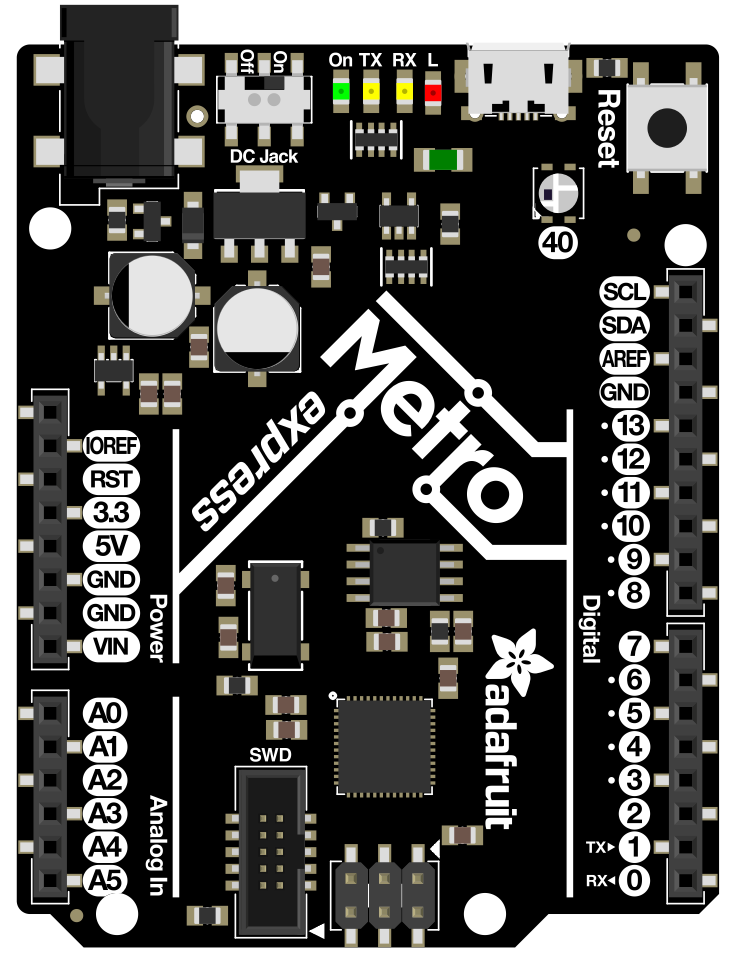
\includegraphics[width=0.438\textwidth]{pics/metro}};
		%%%% Node placement %%%%
		\node [anchor=east] (ref) at (-.3,5.97) {\small I/O Reference voltage};
		\node [anchor=east] (reset) at (-.3,5.593) {\small Reset};
		\node [anchor=east] (lowv) at (-.3,5.217) {\small 3.3V Output};
		\node [anchor=east] (highv) at (-.3,4.84) {\small 5V Output};
		\node [anchor=east] (ground1) at (-.3,4.46) {\small Ground};
		\node [anchor=east] (ground2) at (-.3,4.036) {\small Ground};
		\node [anchor=east] (inputv) at (-.3,3.61) {\small Input voltage};
		%
		\node [anchor=east] (ap0) at (-.3,2.85) {\small Analog pin 0};
		\node [anchor=east] (ap1) at (-.3,2.473) {\small Analog pin 1};
		\node [anchor=east] (ap2) at (-.3,2.096) {\small Analog pin 2};
		\node [anchor=east] (ap3) at (-.3,1.72) {\small Analog pin 3};
		\node [anchor=east] (ap4) at (-.3,1.343) {\small Analog pin 4};
		\node [anchor=east] (ap5) at (-.3,0.966) {\small Analog pin 5};
		%
		% Right side pins
		\node [anchor=west] (scl) at (9,7.78) {\small (I2C) SCL };
		\node [anchor=west] (sda) at (9,7.40) {\small (I2C) SDA};
		\node [anchor=west] (aref) at (9,6.97) {\small Analog Reference voltage};
		\node [anchor=west] (ground3) at (9,6.59) {\small Ground};
		\node [anchor=west] (dp13) at (9,6.21) {\small Digital pin 13, PWM};
		\node [anchor=west] (dp12) at (9,5.83) {\small Digital pin 12, PWM};
		\node [anchor=west] (dp11) at (9,5.45) {\small Digital pin 11, PWM};
		\node [anchor=west] (dp10) at (9,5.07) {\small Digital pin 10, PWM};
		\node [anchor=west] (dp9) at (9,4.69) {\small Digital pin 9, PWM};
		\node [anchor=west] (dp8) at (9,4.31) {\small Digital pin 8, PWM};
		%
		\node [anchor=west] (dp7) at (9,3.62) {\small Digital pin 7};
		\node [anchor=west] (dp6) at (9,3.241) {\small Digital pin 6, PWM};
		\node [anchor=west] (dp5) at (9,2.862) {\small Digital pin 5, PWM};
		\node [anchor=west] (dp4) at (9,2.482) {\small Digital pin 4, PWM};
		\node [anchor=west] (dp3) at (9,2.103) {\small Digital pin 3, PWM};
		\node [anchor=west] (dp2) at (9,1.724) {\small Digital pin 2};
		\node [anchor=west] (tx) at (9,1.345) {\small Communication with computer};
		\node [anchor=west] (rx) at (9,0.966) {\small Communication with computer};
		
		%%%% Arrow placement %%%%
		\draw[-latex, red, ultra thick] (ref) -- (0.60,5.97);
		\draw[-latex, red, ultra thick] (reset) -- (0.6,5.593);
		\draw[-latex, red, ultra thick] (lowv) -- (0.6,5.217);
		\draw[-latex, red, ultra thick] (highv) -- (0.6,4.84);
		\draw[-latex, red, ultra thick] (ground1) -- (0.6,4.46);
		\draw[-latex, red, ultra thick] (ground2) -- (0.6,4.036);
		\draw[-latex, red, ultra thick] (inputv) -- (0.6,3.61);
		%
		\draw[-latex, red, ultra thick] (ap0) -- (0.6,2.85);
		\draw[-latex, red, ultra thick] (ap1) -- (0.6,2.473);
		\draw[-latex, red, ultra thick] (ap2) -- (0.6,2.096);
		\draw[-latex, red, ultra thick] (ap3) -- (0.6,1.72);
		\draw[-latex, red, ultra thick] (ap4) -- (0.6,1.343);
		\draw[-latex, red, ultra thick] (ap5) -- (0.6,0.966);
		% 
		\draw[-latex, red, ultra thick] (scl) -- (8.15,7.78);
		\draw[-latex, red, ultra thick] (sda) -- (8.15,7.40);
		\draw[-latex, red, ultra thick] (aref) -- (8.15,6.97);
		\draw[-latex, red, ultra thick] (ground3) -- (8.15,6.59);
		\draw[-latex, red, ultra thick] (dp13) -- (8.15,6.21);
		\draw[-latex, red, ultra thick] (dp12) -- (8.15,5.83);
		\draw[-latex, red, ultra thick] (dp11) -- (8.15,5.45);
		\draw[-latex, red, ultra thick] (dp10) -- (8.15,5.07);
		\draw[-latex, red, ultra thick] (dp9) -- (8.15,4.69);
		\draw[-latex, red, ultra thick] (dp8) -- (8.15,4.31);
		%
		\draw[-latex, red, ultra thick] (dp7) -- (8.15,3.64);
		\draw[-latex, red, ultra thick] (dp6) -- (8.15,3.241);
		\draw[-latex, red, ultra thick] (dp5) -- (8.15,2.862);
		\draw[-latex, red, ultra thick] (dp4) -- (8.15,2.482);
		\draw[-latex, red, ultra thick] (dp3) -- (8.15,2.103);
		\draw[-latex, red, ultra thick] (dp2) -- (8.15,1.724);
		\draw[-latex, red, ultra thick] (tx) -- (8.15,1.345);
		\draw[-latex, red, ultra thick] (rx) -- (8.15,0.966);
	\end{tikzpicture}
	\caption{Pin-out Diagram for the Adafruit Metro Express.  PWM is Pulse Width Modulation}
	\label{AdafruitPinOut}
\end{figure}


Some pins will not be used for our projects.

\begin{figure}
	\centering
	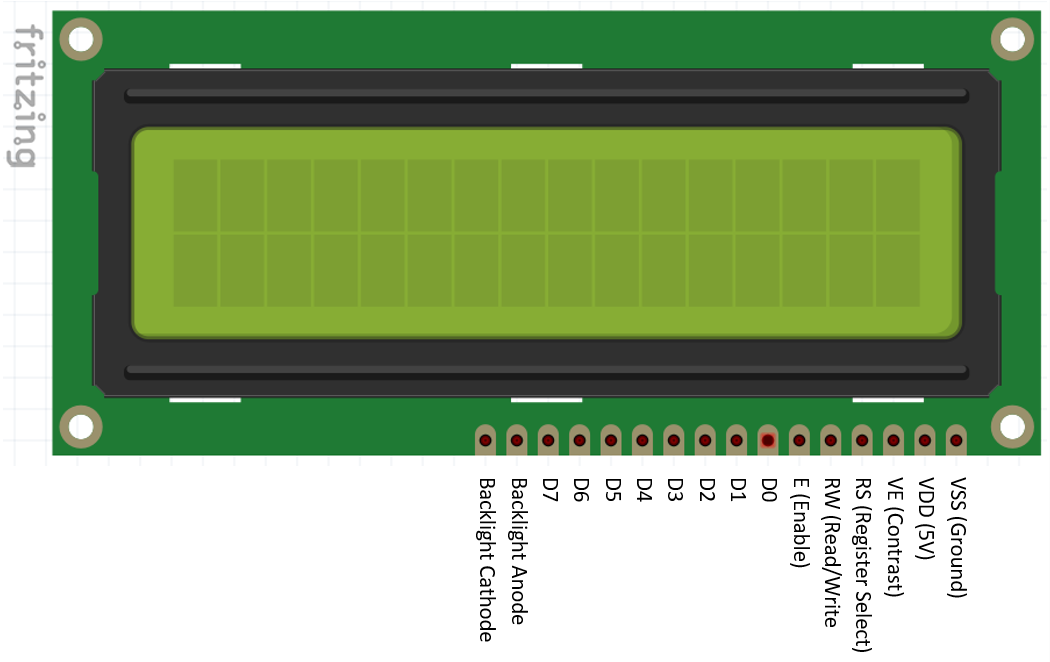
\includegraphics[width=10cm]{pics/lcd pinout.png}
	\caption{Pin-out Diagram for the LCD}
	\label{fig2}
\end{figure}

\begin{figure}
	\centering
	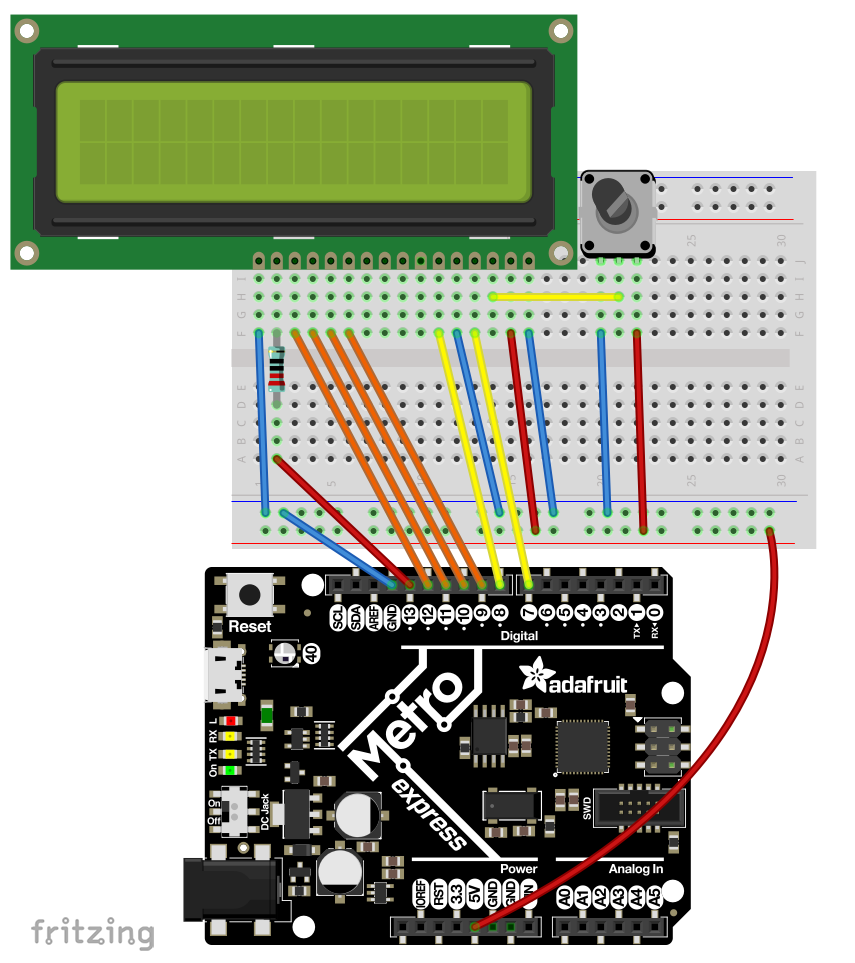
\includegraphics[width=10cm]{pics/lcd wiring.png}
	\caption{Hello World Wiring Diagram}
	\label{HelloWorld}
\end{figure}

The wiring diagram is shown in Figure \ref{HelloWorld}.  It is useful to use the color of wire suggested in the diagram, because it will be  easier to troubleshoot if the board does not work.  It is suggested that you wire the breadboard first (black, red, and blue wires) and then connect the Metro Express with final wires.  

You will need to find a 220$\Omega$ resistor.  The resistance of each resistor is coded on the body  by means of a series of colored bands.  Most resistors have either 4 bands or 5 bands.  See figure \ref{colorchart} for a description of the resistors and the colors used and figure \ref{resistor} for an example of how to read the bands.


\section{Code for the Metro Express}

The code that we will use is written in the computer language "Python", which is often the first programming language students choose to learn.  The code that will be used today is given below.  Note that the text that occurs between 
`````` 
and 
''''''
are comments, not part of the actual code.  Also, any line that begins with \# is a comment. If you delete all of the comments, the code is quite small.

This code is in the file Adafruit\_Basic\_Hello\_World.py.  To open the file for viewing or editing, first save it to your computer. Start the Mu IDE and load the program via the \textit{load} button.  To load the program onto the Metro Express, copy the file into the drive CIRCUITPY and rename it to ``code.py'', overwriting any existing code.py file.  If you load ``code.py'' into the Mu IDE from the CIRCUITPY drive, it will automatically save to that location when you save the file.

The file Adafruit\_Hello\_World.py demonstrates a number of commands available for the LCD.  See \href{https://circuitpython.readthedocs.io/projects/charlcd/en/latest/api.html}{circuitpython.readthedocs.io/projects/charlcd/en/latest/api.html} for a complete list of commands that can be used with the LCD.
\bigskip


\begin{verbatim}
"""
Simple test for monochromatic character LCD

This code is included with the files for Adafruit Labs Hello World by 
Matthew Riehl and is in the public domain.  I have only modified the
code to better support the laboratory exercise.

Demonstrates the use a 16x2 LCD display.  The LiquidCrystal
library works with all LCD displays that are compatible with the
Hitachi HD44780 driver. There are many of them out there, and you
can usually tell them by the 16-pin interface.

This program prints "Hello World!" to the LCD
and shows the number of seconds since reset.


The circuit:
* LCD RS pin to digital pin 7
* LCD Enable pin to digital pin 8
* LCD D4 pin to digital pin 9
* LCD D5 pin to digital pin 10
* LCD D6 pin to digital pin 11
* LCD D7 pin to digital pin 12
* LCD Backlight (pin 15 on LCD) to pin 13 on Adafruit (add a 220 ohm series resistor)
* LCD R/W pin to ground
* LCD VSS pin to ground
* LCD VCC pin to 5V
* 10K potentiostat:
* ends to +5V and ground
* wiper to LCD VO pin (pin 3)

See https://learn.adafruit.com/character-lcds/python-circuitpython for more information.

"""
import time
import board
import digitalio
import adafruit_character_lcd.character_lcd as characterlcd


# Modify this if you have a different sized character LCD
lcd_columns = 16
lcd_rows = 2

# Metro M0/M4 Pin Config:
lcd_rs = digitalio.DigitalInOut(board.D7)
lcd_en = digitalio.DigitalInOut(board.D8)
lcd_d7 = digitalio.DigitalInOut(board.D12)
lcd_d6 = digitalio.DigitalInOut(board.D11)
lcd_d5 = digitalio.DigitalInOut(board.D10)
lcd_d4 = digitalio.DigitalInOut(board.D9)
lcd_backlight = digitalio.DigitalInOut(board.D13)

# Initialise the LCD class
lcd = characterlcd.Character_LCD_Mono(
lcd_rs, lcd_en, lcd_d4, lcd_d5, lcd_d6, lcd_d7, lcd_columns, lcd_rows, lcd_backlight
)

start = time.time()
lcd.clear()
lcd.backlight = True 
lcd.message = "Hello, World!"  # Change this to something cooler.

while True:  # This loop continues forever!
now = time.time()
lcd.message = ('\n{}  seconds'.format(int(now-start)))
\end{verbatim}





\section{Hello World Program in the Mu Editor}

 Connect the Metro Express to the computer with the cable. Open the Mu IDE, identified by the logo shown in Figure \ref{mu}. In the ``Mode'' menu, select \textit{CircuitPython} as the programming mode.  From the ``Load'' dialog, find the CIRCUITPY drive and open it.  There will be one or two .py files: main.py and (probably) code.py.  Code.py is the file that will hold your code and be executed by the micro-controller.  Main.py is a default program that will run if code.py is absent or corrupt.  If code.py is not in the CIRCUITPY drive, you  can drag a .py file to that location and rename it.

 Select code.py to open the file in the Mu editor.  Then, in the same menu, find ``Adafruit\_Basic\_Hello\_World.py'' that you saved to your computer and open that file.  Copy and paste this code into code.py and save this file.  It will save to the Metro Express and immediately begin executing the commands. You may need to adjust the potentiometer to see the display on the LCD.


\begin{figure}[h]
	\centering
	
\includegraphics[width=1cm]{pics/mu.png}
	\caption{Mu Editor Logo}
	\label{mu}
\end{figure}
  

Now, the file Adafruit\_Hello\_World.py can be opened and saved to the code.py file on the CIRCUITPY drive.  Take some time to read the code and try to modify it to see what it can do.  More details on how the commands work can be found online (see the links in the comment section of the program) -- this project is not intended to teach the details of programming.  Rather, it is hoped that you will explore on your own.


	\begin{figure}
	\begin{center}
		\renewcommand*{\arraystretch}{1.2}
		\begin{tabular}{cccccc}
			\hline
			Color & \(1^{\text{st}}\) Band & \(2^{\text{nd}}\) Band & \(3^{\text{rd}}\) Band & Multiplier & Tolerance \\ \hline
			\rowcolor{black} \tc{white}{\textbf{Black}} & \tc{white}{0} & \tc{white}{0} & \tc{white}{0} & \tc{white}{\(1 \Omega\)} &  \\
			\rowcolor{brown} \textbf{Brown} & 1 & 1 & 1 & \(10 \Omega\) & \(\pm 1\%\) \\
			\rowcolor{red} \textbf{Red} & 2 & 2 & 2 & \(100 \Omega\) & \(\pm 2\%\) \\
			\rowcolor{orange} \textbf{Orange} & 3 & 3 & 3 & \(1 \text{k}\Omega\) &  \\
			\rowcolor{yellow} \textbf{Yellow} & 4 & 4 & 4 &\(10 \text{k}\Omega\)  &  \\
			\rowcolor{green} \textbf{Green} & 5 & 5 & 5 & \(100 \text{k}\Omega\) & \(\pm 0.5\%\) \\
			\rowcolor{blue} \tc{white}{\textbf{Blue}} & \tc{white}{6} & \tc{white}{6} & \tc{white}{6} & \tc{white}{\(1 \text{M}\Omega\)} & \tc{white}{\(\pm 0.25\%\)} \\
			\rowcolor{violet} \tc{white}{\textbf{Violet}} & \tc{white}{7} & \tc{white}{7} & \tc{white}{7} & \tc{white}{\(10 \text{M}\Omega\)} & \tc{white}{\(\pm 0.10\%\)} \\
			\rowcolor{black!50} \tc{white}{\textbf{Grey}} & \tc{white}{8} & \tc{white}{8} & \tc{white}{8} & \tc{white}{\(100 \text{M}\Omega\)} & \tc{white}{\(\pm 0.05\%\)} \\
			\rowcolor{white} \textbf{White} & 9 & 9 & 9 & \(1 \text{G}\Omega\) &  \\
			\rowcolor{Dandelion} \textbf{Gold} &  &  &  & \(0.1 \Omega\) & \(\pm 5\%\) \\
			\rowcolor{black!25} \textbf{Silver} &  &  &  & \(0.01 \Omega\) & \(\pm 10\%\) \\ \hline
		\end{tabular}
		\caption{Color banding codes for resistors}
		\label{colorchart}
	\end{center}
	\end{figure}

	\begin{figure}
		\centering
		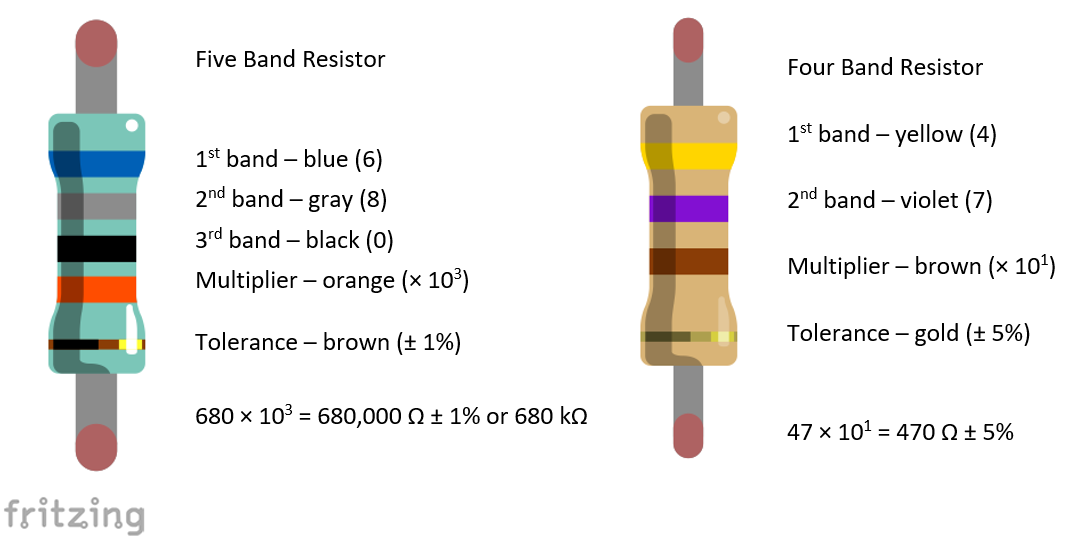
\includegraphics[width=12cm]{pics/resistor.png}
		\caption{Examples of a 5-band and 4-band resistor}
		\label{resistor}
	\end{figure}

\end{document}
